%\onecolumn
\setcounter{equation}{0}
\renewcommand\theequation{A.\arabic{equation}}
\section*{A}
\label{sec:appendix}

Here are figures of data we gathered, but didn't end up using. Most of them are zoomed in cases, but we also include the mean magnetisation.

\begin{figure}[htbp]
	\centering
	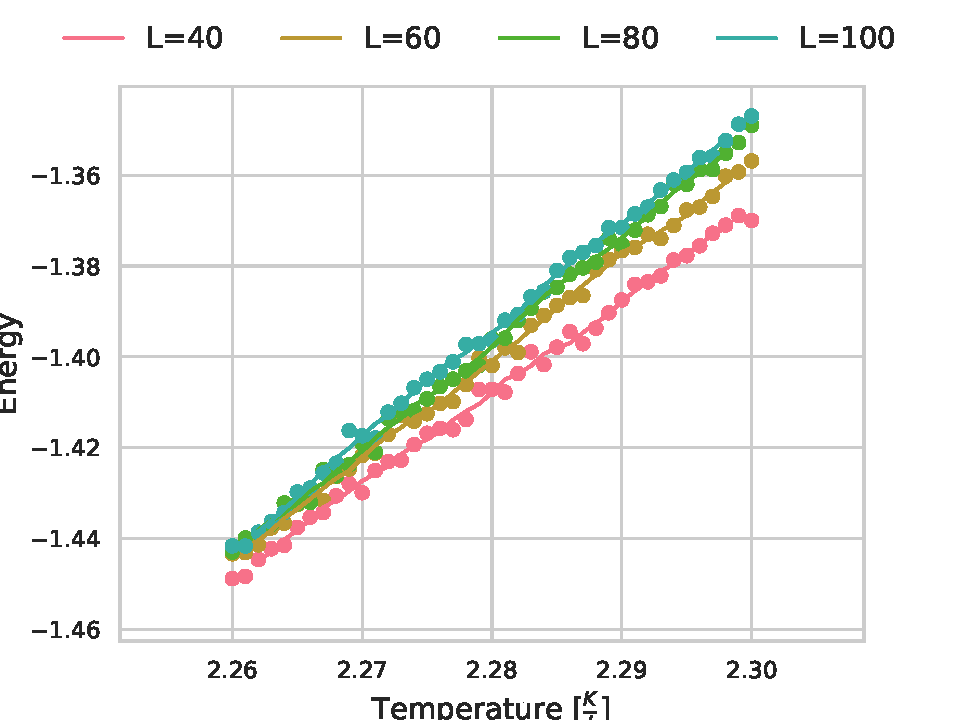
\includegraphics[width=0.5\textwidth]{Energy0001.pdf}
	\caption{Mean energy as a function of temperature $T\in[2.26, 2.3]$ for lattice sizes $L= 40, 60, 80, 100$, with a rolling mean, window size 5.}
\end{figure}

\begin{figure}[htbp]
	\centering
	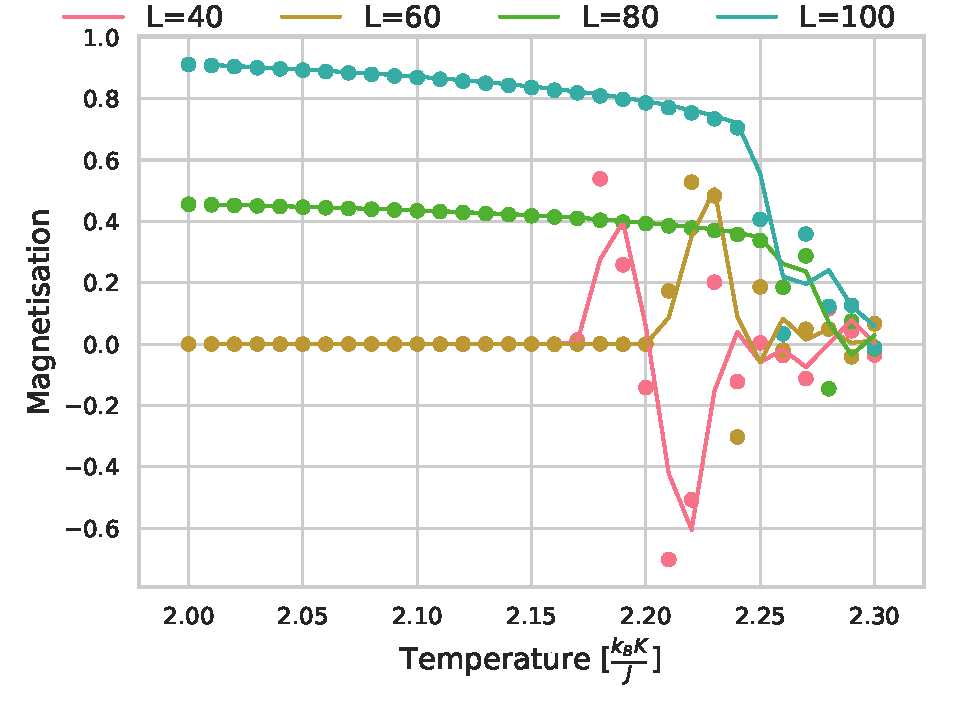
\includegraphics[width=0.5\textwidth]{Magnetisation001.pdf}
	\caption{Mean magnetisation as a function of temperature $T\in[2.0, 2.3]$ for lattice sizes $L= 40, 60, 80, 100$, with a rolling mean, window size 2.}
\end{figure}

\begin{figure}[htbp]
	\centering
	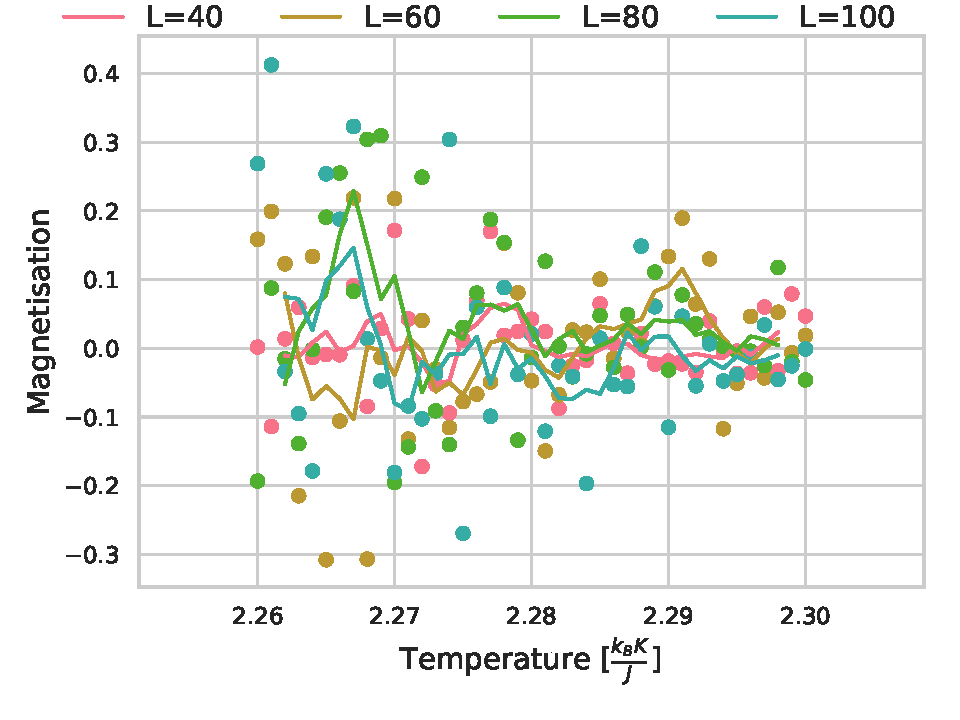
\includegraphics[width=0.5\textwidth]{Magnetisation0001.pdf}
	\caption{Mean magnetisation as a function of temperature $T\in[2.26, 2.3]$ for lattice sizes $L= 40, 60, 80, 100$, with a rolling mean, window size 5.}
\end{figure}

\begin{figure}[htbp]
	\centering
	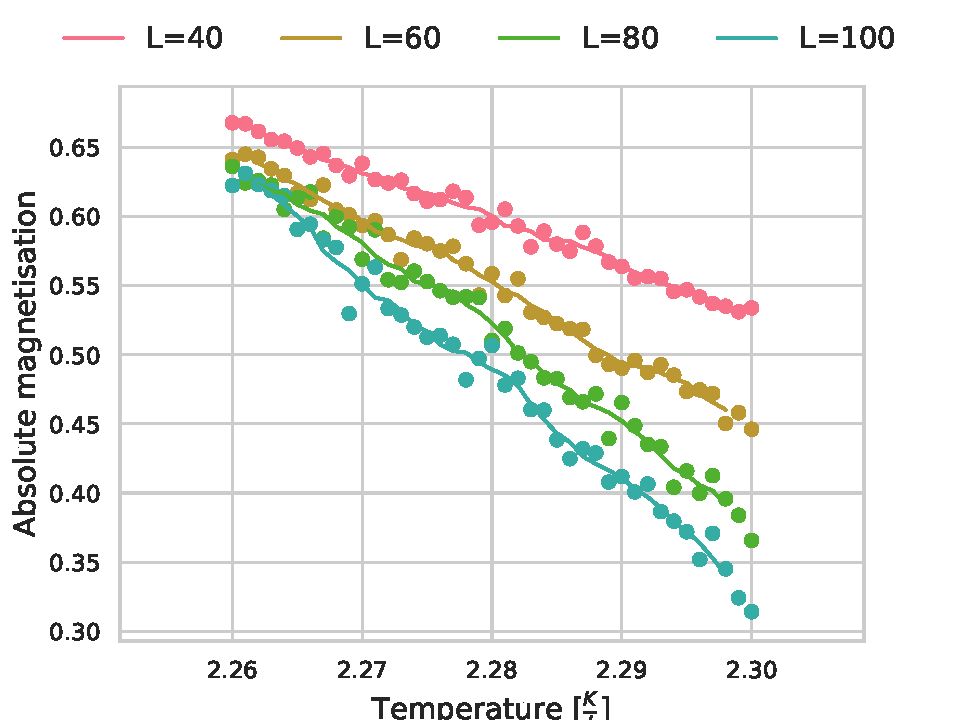
\includegraphics[width=0.5\textwidth]{Absolute_magnetisation0001.pdf}
	\caption{Absolute magnetisation as a function of temperature $T\in[2.26, 2.30]$ for lattice sizes $L= 40, 60, 80, 100$, with a rolling mean, window size 5.}
\end{figure}

\begin{figure}[htbp]
	\centering
	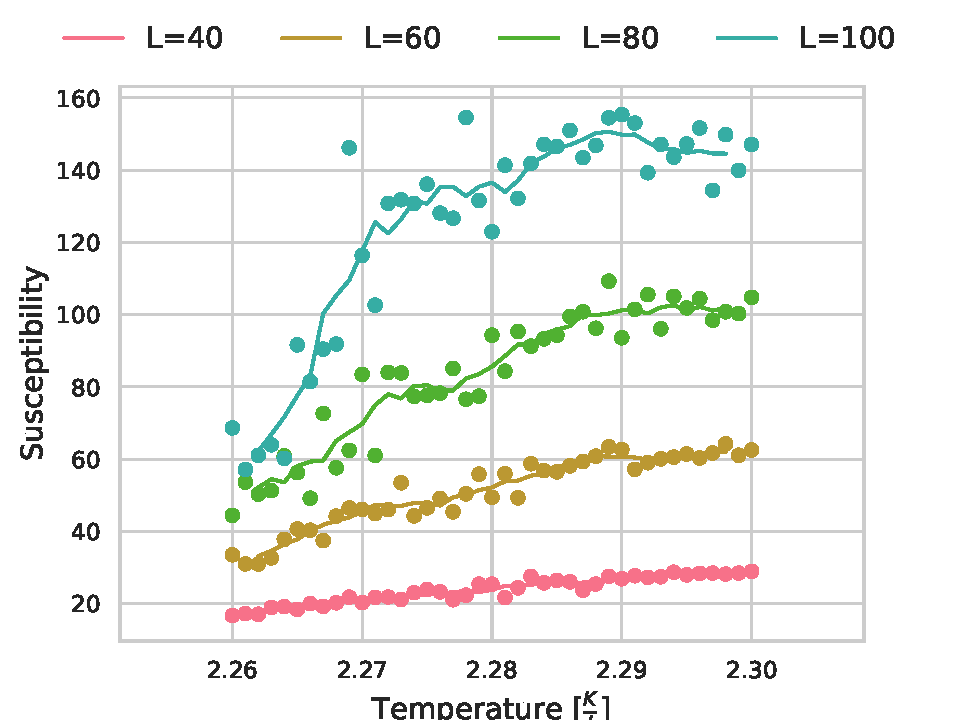
\includegraphics[width=0.5\textwidth]{Susceptibility0001.pdf}
	\caption{Susceptibility as a function of temperature $T\in[2.26, 2.30]$ for lattice sizes $L= 40, 60, 80, 100$, with a rolling mean, window size 5.}
\end{figure}
